\documentclass[12pt]{article}
\usepackage{caption}
\usepackage{subcaption}
\usepackage{graphicx}
\graphicspath{ {images/} }
\usepackage{geometry}
\usepackage{pdfpages}
\usepackage{array}
\usepackage{amsmath}
\usepackage{url}
\usepackage[portuguese]{babel}
%opening
\title{Exercícios de Fixação de Conceitos 1 - EFC1 - IA048}
\author{Marcelo Eduardo Pederiva RA: 122580}
\date{}
\geometry{total={210mm,297mm},
	left=20mm,right=20mm,
	bindingoffset=10mm, top=0mm,bottom=20mm}

\begin{document}

\maketitle
\section*{Parte 1 - Atividades Teóricas}

\subsection*{Exercício 1}
\subsubsection*{a)}


\begin{align*}
	P(X) = \sum_xP(X=x))
\end{align*}

\begin{align*}\
	&P(X=0) = P(X=0,Y=0)+P(X=0,Y=1)\\
	&P(X=0) = 0.5+0.05
\end{align*}

\begin{equation*}
	\boxed{P(X=0) = 0.55}
\end{equation*}

\begin{align*}\
	&P(X=1) = P(X=1,Y=0)+P(X=1,Y=1)\\
	&P(X) = 0.3+0.15
\end{align*}

\begin{equation*}
\boxed{P(X=1) = 0.45}
\end{equation*}

\begin{align*}
P(Y) = \sum_yP(Y=y))
\end{align*}

\begin{align*}\
	&P(Y=0) = P(Y=0,X=0)+P(Y=0,X=1)\\
	&P(Y=0) = 0.5+0.3
\end{align*}
\begin{equation*}
\boxed{P(Y=0) = 0.8}
\end{equation*}


\begin{align*}\
	&P(Y=1) = P(Y=1,X=0)+P(Y=1,X=1)\\
	&P(Y=1) = 0.05+0.15
\end{align*}
\begin{equation*}
\boxed{P(Y=1) = 0.2}
\end{equation*}

\newgeometry{left=3cm, right = 2cm, textwidth=12cm,top=1.5cm,bottom=2cm,heightrounded}

\subsubsection*{b)}
\begin{align*}
	&P(X=1|Y=1) = \frac{P(Y=1,X=1)}{P(Y=1)}\\
	&P(X=1|Y=1) =\frac{0.15}{0.2}
\end{align*}
\begin{equation*}
\boxed{P(X=1|Y=1) = 0.75}
\end{equation*}

\subsubsection*{c)}
Para observar se as variáveis são descorrelacionadas vamos calcular a $cov(X,Y)$. Se $cov(X,Y) = 0$, temos que as variáveis são descorrelacionadas.

\begin{align*}
	cov(X,y) &= E[(X-\mu_x)-(Y-\mu_y)]\\
			 &= \sum_{x,y}(x -\mu_x)-(y -\mu_y)P()X=x,Y=y)
\end{align*}

\begin{align*}
	\mu_x = 0*0,5+0*0,05+1*0,3+1*0,15 = 0,45\\
	\mu_y = 0*0,5+0*0,3+1*0,0,5+1*0,15 = 0,20
\end{align*}

Dessa forma temos,

\begin{align*}
	cov(X,Y) &= (0-0,45)(0-0,2)0,5 + (0-0,45)(1-0,2)0,5 \\
			 &+ (1-0,45)(0-0,2)0,5 + (1-0,45)(1-0,2)0,5\\
	cov(X,Y) &= 0,045-0,018-0,033+0,66 \\
	cov(X,Y) &= 0,06 \neq 0
\end{align*}

Assim temos que as variáveis são correlacionadas.

\subsubsection*{d)}

Temos que, para uma variável ser independente, ela deve satisfazer as seguintes condições:
\begin{itemize}
	\item $P(X|Y) = P(X)$ para todos valores de X e Y.
	
	\item $P(X \cap Y) = P(X)*P(Y)$ para todos valores de X e Y.
\end{itemize}

Através dos resultados obtidos pelo item a) e b) temos que,
\begin{align*}
	P(X=1|Y=1) = 0.75 \neq 0.45 = P(X=1)
\end{align*}


Sendo assim podemos admitir que as duas variáveis não são independentes.


\subsubsection*{e)}
\begin{itemize}
	\item{\large $H(X)$}
\end{itemize}


\begin{align*}
	H(X) &= - \sum_{x}P(X=x)\log_2[P(X=x)]\\
		& = -(P(X=0)\log_2[P(X=0)] + P(X=1)\log_2[P(X=1)])\\
		& = 0,55(-0,8625) + 0,45(-1,1520)
\end{align*}
\begin{equation*}
\boxed{H(X) = 0,9928}
\end{equation*}
\vspace{2cm}
\begin{itemize}
	\item{\large $H(Y)$}
\end{itemize}


\begin{align*}
	H(Y) &= - \sum_{y}P(Y=y)\log_2[P(Y=y)]\\
		& = -(P(Y=0)\log_2[P(Y=0)] + P(Y=1)\log_2[P(Y=1)])\\
		& = -(0,8(-0,3219) + 0,2(-2,3219))
\end{align*}
\begin{equation*}
\boxed{H(Y) = 0,7219}
\end{equation*}
\vspace{2cm}
\begin{itemize}
	\item{\large $H(X,Y)$}
\end{itemize}


\begin{align*}
H(X,Y) = &- \sum_{x}\sum_{y}P(X=x,Y=y)\log_2[P(X=x,Y=y)]\\
	   = &- ( P(X=0,Y=0)\log_2[P(X=0,Y=0)] + P(X=0,Y=1)\log_2[P(X=0,Y=1)]  \\
	     &+   P(X=1,Y=0)\log_2[P(X=1,Y=0)] + P(X=1,Y=1)\log_2[P(X=1,Y=1)])\\
H(X,Y) = &-(0,5\log_2(0,5) + 0,05\log_2(0,05) + 0,3\log_2(0,3) + 0,15\log_2(0,15))
\end{align*}
\begin{equation*}
\boxed{H(X,Y) = 1,6477}
\end{equation*}
\vspace{2cm}

\begin{itemize}
	\item{\large $H(X|Y)$}
\end{itemize}


\begin{align*}
H(X,Y) =& H(Y) + H(X|Y)\\
H(X|Y) =& H(X,Y) - H(Y)\\
H(X|Y) =& 1,6477 - 0,7219
\end{align*}
\begin{equation*}
\boxed{H(X|Y) = 0,9258}
\end{equation*}

\vspace{2cm}
\begin{itemize}
	\item{\large $H(Y|X)$}
\end{itemize}


\begin{align*}
H(X,Y) =& H(X) + H(Y|X)\\
H(Y|X) =& H(X,Y) - H(X)\\
H(Y|X) =& 1,6477 - 0,9928
\end{align*}
\begin{equation*}
\boxed{H(Y|X) = 0,6549}
\end{equation*}
\vspace{2cm}
\subsubsection*{f)}
\begin{align*}
	I(X,Y) =& H(X) - H(X|Y) = H(Y) - H(Y|X)\\
	I(X,Y) =& 0,9928 - 0,9258 
\end{align*}
\begin{equation*}
	\boxed{I(X,Y) = 0,067}
\end{equation*}
\pagebreak

\section*{Parte 2 - Atividade Computacional}

\subsection*{Exercício 1}

Neste primeiro exercício, utilizamos um aproximador linear para prever o valor médio de manchas solares nos próximos meses. Para isso, foi separado os últimos dez anos de dados (2010-2019) como conjunto de teste. Da mesma forma, os dados restantes foram usados como conjunto de treinamento.

Na etapa de treinamento, foi utilizado o método de validação cruzada. Para isso, determinando 20\% do conjunto de treinamento como dados de validação, foi utilizado 5 "pastas" para realizar a validação cruzada do treinamento.

\subsubsection*{1.}
Nesta etapa, observamos a influência no erro da predição quando aumentamos a quantidade de meses anteriores utilizados no treinamento.

\begin{figure}[h!]
	\centering
	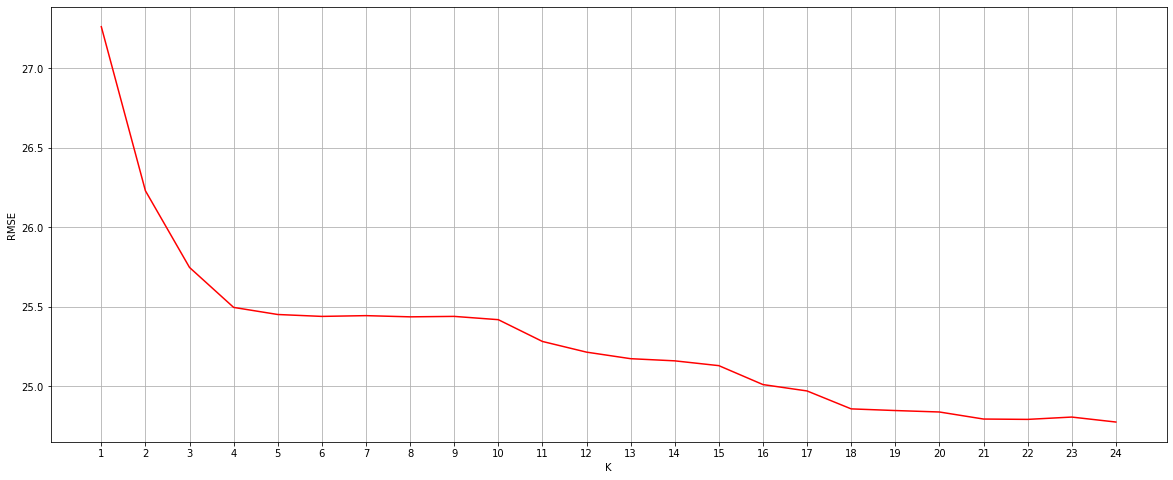
\includegraphics[width=\linewidth]{rmse_vs_k.png}
	\caption{Relação do erro na predição com o valor K.}
	\label{fig:rmse_vs_k}
\end{figure}

Como podemos observar na Figura \ref{fig:rmse_vs_k}, o aumento de meses anteriores nos dados teve uma influência positiva na predição do valor médio de manchas solares no próximo mês.

Neste treinamento o menor valor médio da raiz quadrada do erro quadrático médio (RMSE, do inglês \textit{root mean squared error}) da predição alcançou um valor de \textbf{RMSE=24.7761}  com  \textbf{K = 24}. 



\pagebreak
\subsubsection*{2.}

Dessa forma, utilizando a matriz $W$ treinada com o K= 24, prevemos os valores do conjunto de teste e comparamos com os valores reais esperados (Figura \ref{fig:test_k_24}).

\begin{figure}[h!]
	\centering
	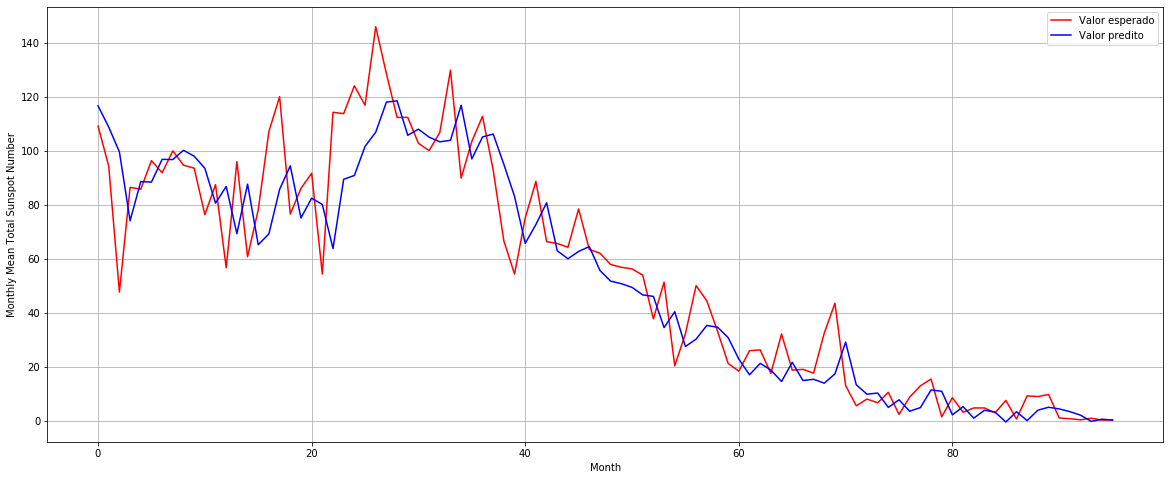
\includegraphics[width=\linewidth]{test_k_24.png}
	\caption{Comparação do valor predito com o valor esperado.}
	\label{fig:test_k_24}
\end{figure}

Podemos observar, que a curva predita tem uma boa aproximação da curva esperada, entretanto, possui um deslocamento a direita dos dados reais. Isto pode ocorrer pelo preditor linear valorizar mais os meses mais próximos da predição, ou seja, os meses meses mais recentes recebem um peso maior na matriz W. Dessa forma, a predição sempre propõe um valor próximo ao apresentado no mês anterior. 

Por fim, o Preditor Linear alcançou um valor de \textbf{RMSE = 15.8979} no conjunto de teste.

\subsection*{Exercício 2}

Neste exercício, implementamos uma aproximação não-linear para resolução do mesmo problema. Para isso, os dados que utilizamos para treinar o modelo sofreu um preprocessamento, uma normalização, seguido por uma multiplicação com uma matriz com números uniformemente aleatórios ($W_k$) e posteriormente aplicamos a tangente hiperbólica nesse resultado (Equação \ref{eq1}). 

\begin{equation}
	x'_k(n) = tanh(\textbf{W}_k^T\textbf{x}_{norm}(n))
	\label{eq1}
\end{equation}

Os dados foram normalizados para valores entre 0 e 0,5 e a matriz $W_k$ foi gerada por números uniformemente aleatórios entre 0 e 0,5.

Para avaliar os resultados da predição não-linear em comparação com da predição linear, foi utilizado o mesmo método de validação cruzada com 5 "pastas".

\pagebreak
\subsubsection*{a)}

Tendo como base o K=8, iremos observar a influência do tamanho da matriz ($W_k$) no erro de predição (RMSE) junto aos dados de validação.

\begin{figure}[h!]
	\centering
	\includegraphics[width=\linewidth]{rmse_vs_T.png}
	\caption{Erro de validação de cada valor de T, ponto vermelho representa o T com menor RMSE.}
	\label{fig:rmse_vs_t}
\end{figure}

Como podemos observar na Figura \ref{fig:rmse_vs_t}, o aumento do número de atributos (T) proporciona um menor erro nas predições de validação. Sendo assim, com o K=8, obtivemos o menor \textbf{RMSE = 25.4811} com \textbf{T = 87}.


\subsubsection*{b)}

A seguir, iremos observar a variação do termo de regularização para cada T. Este coeficiente foi variado entre $2^{-10}$ a $2^{10}$ para cada T, onde foi destacado o coeficiente que gerava o menor erro de validação. Podemos observar pela Figura \ref{fig:c_vs_t} o melhor valor do termo de regularização para cada número de atributos.


\begin{figure}[h!]
	\centering
	\includegraphics[width=\linewidth]{c_vs_t.png}
	\caption{Melhor coeficiente de regularização para cada T.}
	\label{fig:c_vs_t}
\end{figure}

Assim, tendo T=87 como melhor candidato proposto pelo item a), encontramos que o melhor coeficiente de regularização para este T é o valor \textbf{0.0078125}.

\subsubsection*{c)}
Por fim, utilizando os melhores resultados dos itens anteriores geramos um estimador não-linear para prever o conjunto de teste. 

\begin{figure}[h!]
	\centering
	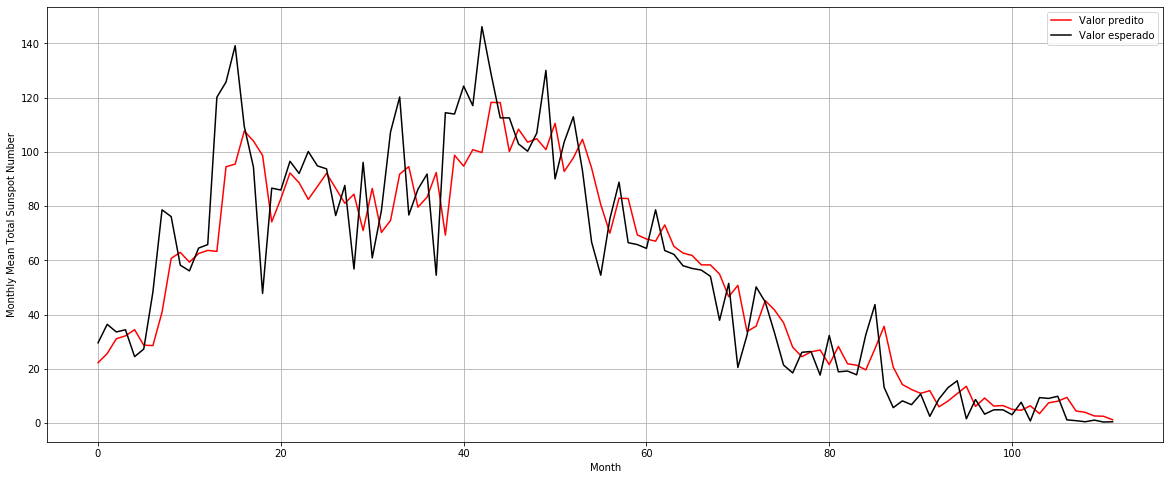
\includegraphics[width=\linewidth]{test_best.png}
	\caption{Comparação do valor predito com o valor esperado.}
	\label{fig:test_best}
\end{figure}

Esta configuração de Ridge Regression resultou em um \textbf{RMSE = 16.7270}. 
\pagebreak
\subsection*{Conclusão}

Neste trabalho utilizei meu RA (122580) como "\textit{seed}" para gerar os números aleatórios da matriz $W_k$, outras "\textit{seeds}" podem resultar numa pequena variação da predição não-linear. Também foi variado tanto os valores de normalização, como o intervalo de números aleatórios gerados pela matriz $W_k$. Os valores definidos no trabalho final foram os que retornaram menores erros junto aos dados de validação. 

Por fim, o preditor não-linear apresentou um resultado próximo ao do preditor linear. Comparando os dois métodos com o mesmo K (K=8), observamos o seguinte resultado:

\begin{center}
	Preditor Linear \hspace{1.8cm}  RMSE = 16.5682 
	
	Preditor Não-Linear \hspace{1cm}  RMSE = 16.7270 
\end{center}

Também podemos observar na Figura \ref{fig:compare_test} os valores preditos de cada estimador, preditor linear em azul, preditor não-linear em vermelho e valor esperado em preto.

\begin{figure}[h!]
	\centering
	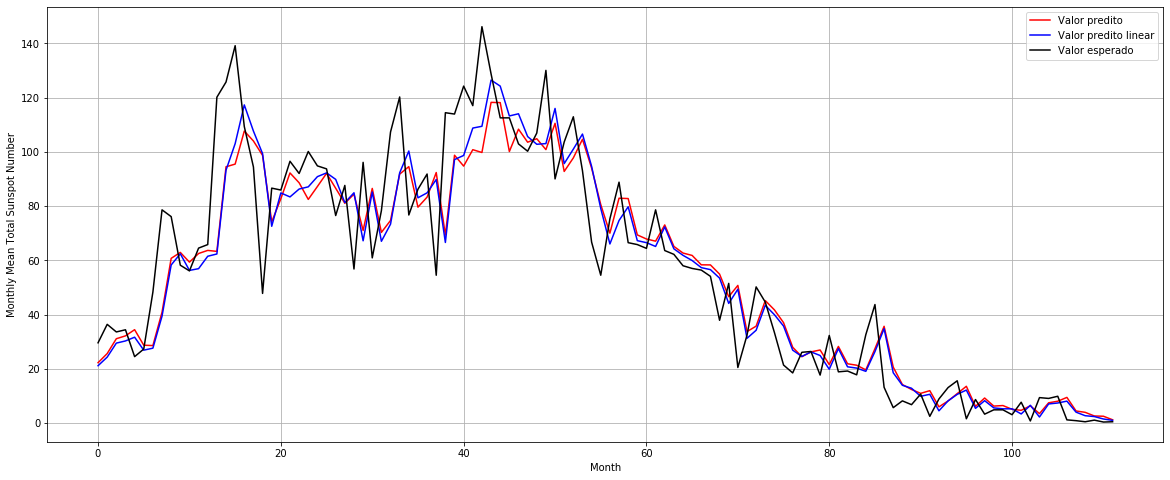
\includegraphics[width=\linewidth]{compare_test.png}
	\caption{Comparação dos Preditores junto aos dados de Teste, com K=8.}
	\label{fig:compare_test}
\end{figure}

Apesar de ser possível encontrar um resultado levemente superior para o preditor não-linear, com outros números aleatórios gerados pela matriz $W_k$, observamos que o preditor linear satisfaz a predição desta serie não-estacionária de forma satisfatória e equivalente à de um preditor não-linear.

\end{document}
